\documentclass{article}

\usepackage{float}
\usepackage{amsmath}
\usepackage{graphicx}
\usepackage{booktabs}

\title{Assignment of ET 4389}
\author{Volker Strobel}
\date{\today}

\begin{document}
\maketitle

I'm a guest student from the Radboud University. My TU Delft student
number is 4524187, my official start date at the TU Delft is March
2016, however, I have not received my login credentials
yet. Therefore, I've used my employee account (I'm also doing an
internship here) for this assignment.

\subsection*{1)}
$G$ is the network described in \texttt{7.txt}.

\begin{itemize}
  \item Number of nodes $N$: $379$ 
  \item Number of links $L$: $914$
  \item Link density $p$: $0.013$
  \item Average degree $E[D]$: $4.82$
  \item Degree variance $Var[D]$: $15.46$
\end{itemize}
The degree distribution of $G$ is shown in
Figure~\ref{fig:degree-distribution}.
\begin{figure}[H]
  \centering
  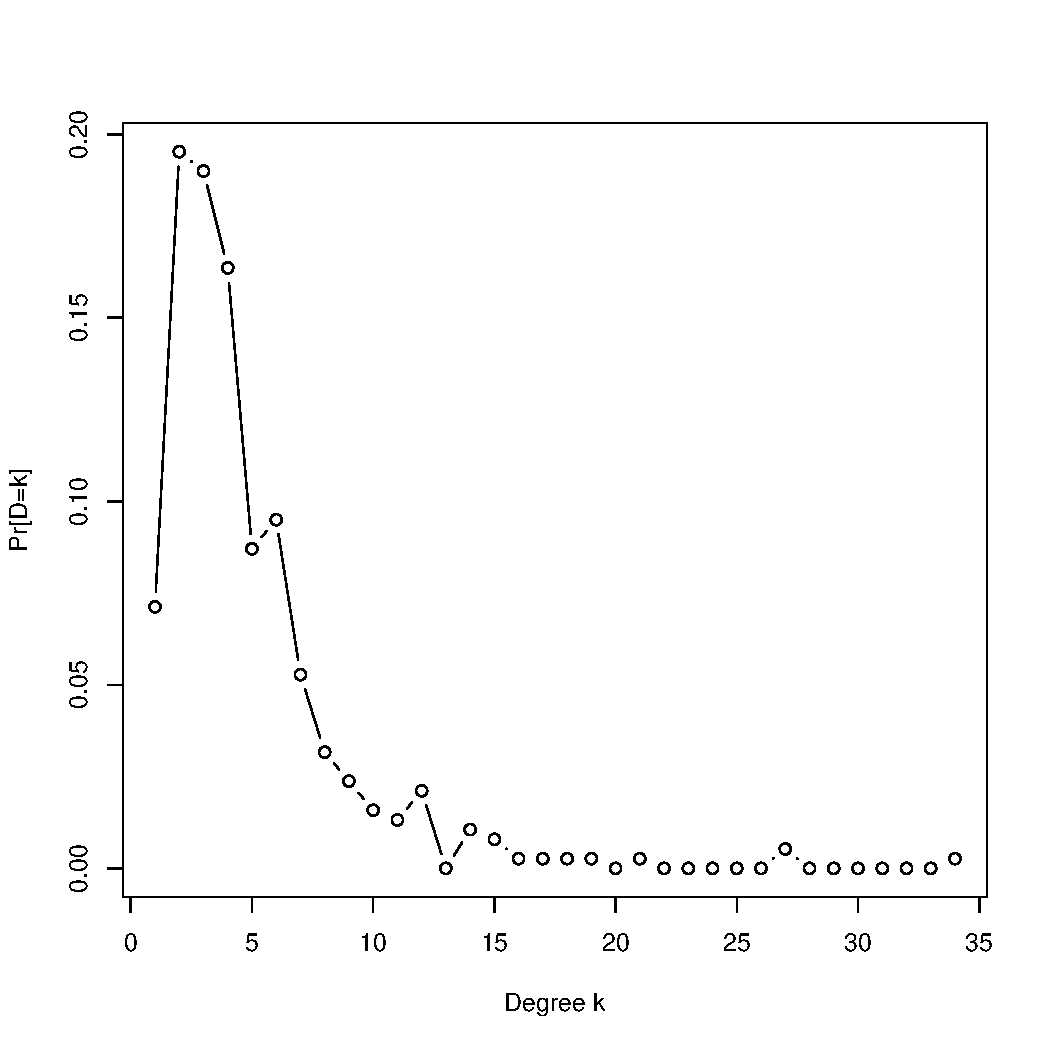
\includegraphics[width=0.75\textwidth]{degree_distribution_1}
  \caption{Degree distribution of Graph $G$}
  \label{fig:degree-distribution}
\end{figure}

The power law distribution has been fit using a linear regression,
with the logarithm of the degree as the predictor and the logarithm of
the probability as target value.

As can be seen in Figure~\ref{fig:fitted-curve}, the degree
distribution roughly follows a power law distribution; however,
especially degree 1 is far off the fit power law curve. The obtained
values are: $\gamma = - 1.55$ and $c = 0.61$.

\begin{figure}[H]
  \centering
  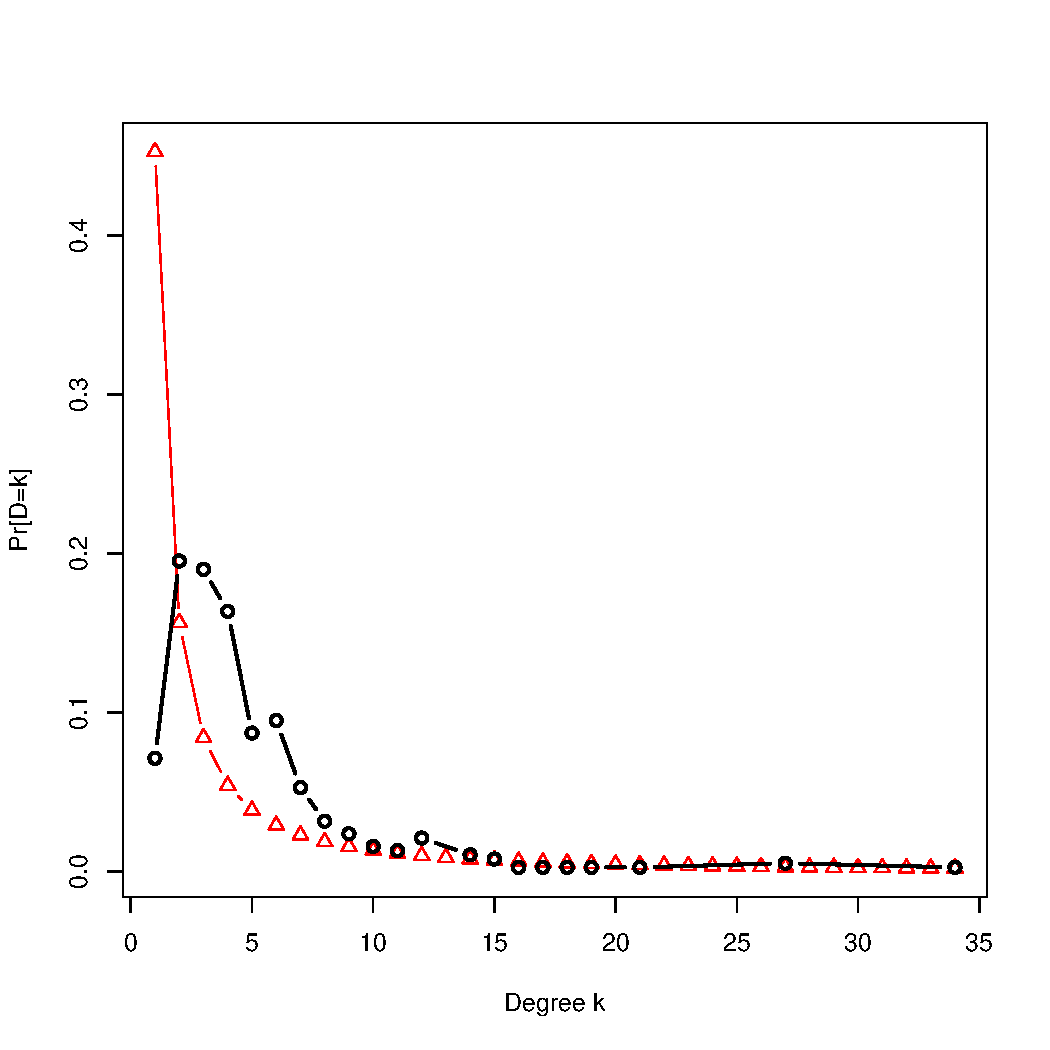
\includegraphics[width=0.75\textwidth]{fitted_curve_normalized}
  \caption{Fitting curve for graph $G$, with power exponent $\gamma =
    - 1.55$ and $c = 0.61$.}
  \label{fig:fitted-curve}
\end{figure}

\subsection*{2)}

\begin{itemize}
\item Degree correlation (assortativity) $\rho_D$: $-0.30$
\end{itemize}
Networks, in which nodes with a high degree are likely connected to
other high-degree nodes and nodes with a low degree are are likely
connected to other low-degree nodes are \emph{assortative} and have a
positive $\rho_D$ (\emph{Birds of a feather flock together}). Networks
in which nodes with a low degree are likely connected to high-degree
nodes are \emph{disassortative} and have a negative $\rho_D$
(\emph{Opposites attract.}).

\subsection*{3)}

\begin{itemize}
  \item Clustering coefficient: $0.17$
\end{itemize}

\subsection*{4)}

\begin{itemize}
  \item Average hopcount $E[H]$: $3.75$
  \item Diameter $H_{max}$: $7$
\end{itemize}

\subsection*{5)}
\begin{itemize}
  \item Largest eigenvalue (spectral radius) $\lambda_1$: $7.44$
\end{itemize}
\subsection*{6)}

\begin{itemize}
\item Second smallest eigenvalue (algebraic connectivity) of the
  Laplacian matrix $\mu_{N-1}$: $0.40$
\end{itemize}

\subsection*{7)}
Now, we consider the network $G_N$, described in \texttt{NetScience.txt}.

\begin{itemize}
\item Number of nodes $N$: $379$
\item Number of links $L$: $914$
\item Link density $p$: $0.013$
\item Average degree $E[D]$: $4.82$
\item Degree variance $Var[D]$: $15.46$
\item Clustering coefficient $C$: $0.80$
\item Assortativity $\rho_D$: $-0.08$
\item Average hopcount $E[H]$: $6.04$
\item Spectral radius $\lambda_1$: $10.38$
\item Algebraic connectivity $\mu_{N-1}$: $0.015$
\item Diameter $H_{max}$: $17$
\end{itemize}

\subsection*{8)}

\noindent\emph{Clustering coefficient $C$}. The clustering coefficient $C$
states how densely the neighbors of an agent are connected with each
other. Here, $G_N$ has a much higher coefficient $C$ ($C(G) = 0.17 <
C(G_N) = 0.80$), which is typical for a real-world network. Clustering
can form some robustness against attacks (since information can be
passed among the neighbors of an agent on several channels) but can
also mean that information is primarily spread within a certain clique
without too much contact to agents outside of the clique. Therefore,
no design has a clear advantage here.

\vspace*{0.5em}
\noindent
\emph{Average hopcount E[H]}. The average hopcount states the expected
length of the shortest path between two nodes. This can be interpreted
as the delay of the communication network. The smaller the average
hopcount, the smaller the delay, and the faster messages can be sent
between two partners. Since the average hopcount of $G$ is $3.75$,
messages can be sent much faster than in $G_N$ with $E[H] = 6.04$.

\vspace*{0.5em}
\noindent\emph{Diameter $H_{max}$}. The diameter of the communication network
states how many edges a message needs to pass between the sender and
the receiver in the worst case. Since a smaller $H_{max}$ means faster
communication in the worst case, $G$ performs better ($H_{max}(G) = 7
< H_{max}(G_N) = 17$).

\vspace*{0.5em}
\noindent\emph{Spectral radius $\lambda_1$}.
The spectral radius is important for dynamic processes in networks,
for example, if, and when, a message might go ``viral'', and receive
as many participants as possible. The larger $\lambda_1$, the lower
the epidemic threshold $\tau_c$. Therefore, for fast widespread
information propagation, a higher $\lambda_1$ can be beneficial,
therefore, $G_N$ performs better ($\lambda_1(G) = 7.44 <
\lambda_1(G_N) = 10.38$).

\vspace*{0.5em}
\noindent%
\emph{Algebraic connectivity $\mu_{N-1}$}. This metric states how well
connected a graph is: the larger $\mu_{N-1}$, the more difficult it is
to disconnect or split apart the communication network -- therefore a
high $\mu_{N-1}$ shows more robustness in case of failures or
breakdown of links. If the value is greater than zero, the graph is a
connected graph -- this is important in a communication framework to
analyze if a certain message can reach each participant. Since $G$ has
the higher connectivity, it performs better ($\mu_{N-1}(G) = 0.40 >
\mu_{N-1}(G_N) = 0.015$).

\vspace*{0.5em}
\noindent All in all, I would recommend design $G$. It offers a
shorter average and maximum delay for messages, which is better suited
to quickly conveying information across the network.  Additionally, it
shows a higher algebraic connectivity and is, therefore, potentially
more robust in case of failures. However, fast widespread information
propagation might be better in $G_N$, therefore, the choice of the
model depends on the final application.

\subsection*{9)}

\begin{figure}[H]
  \centering
  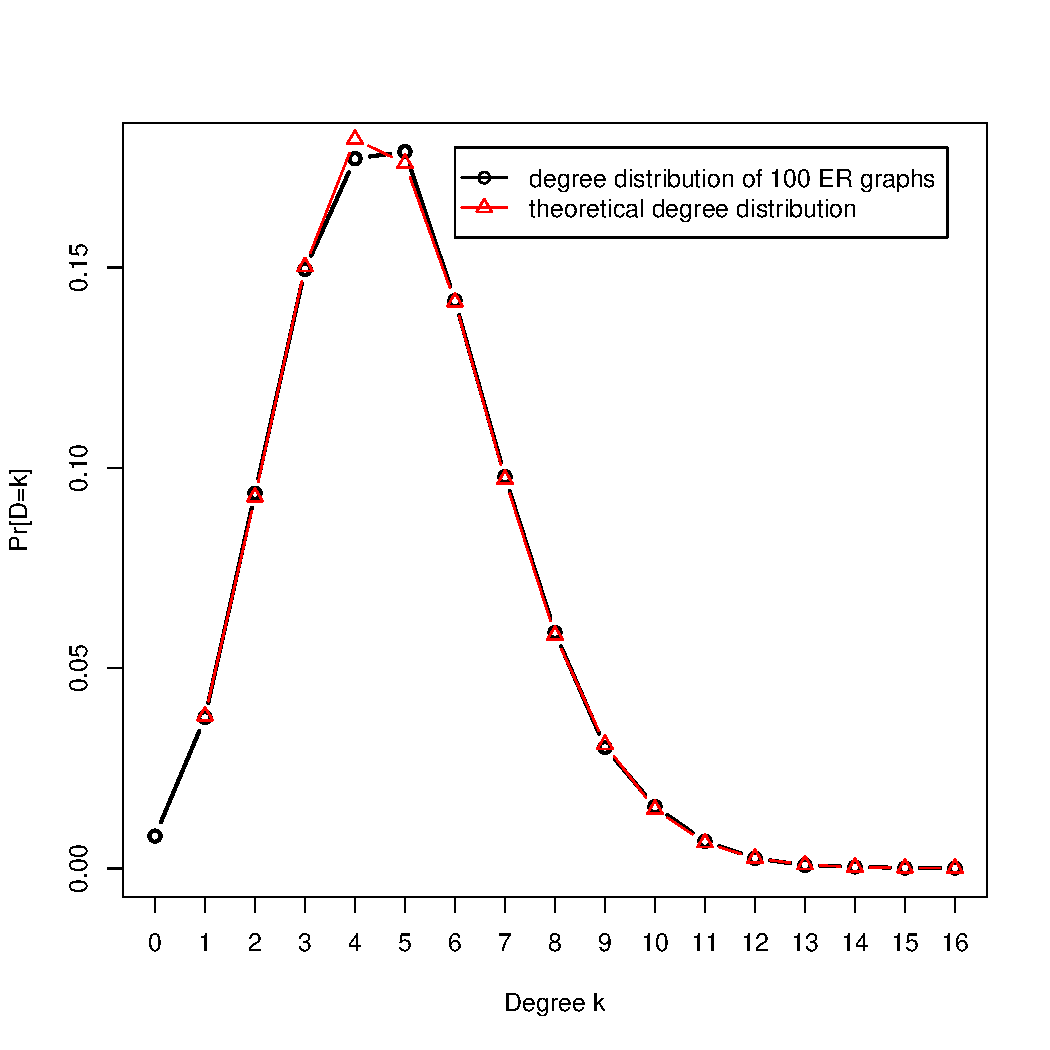
\includegraphics[width=0.7\textwidth]{er_degree_distribution}
  \caption{Comparison of the degree distribution of 100 ER instances
    and the theoretical degree distribution, where $Pr[D=k] =
    \binom{N-1}{k}p^k(1-p)^{N-1-k}=\binom{378}{k}0.013^k\cdot0.987^{378-k}$.}
\end{figure}


\subsection*{10)}
Average of the metrics over the 100 ER random networks:
\begin{itemize}
 \item Number of nodes $N$: 379
 \item Number of links $L$: 914.33
 \item Link density $p$: 0.013
 \item Average degree $E[D]$: 4.82
 \item Degree variance $Var[D]$: 4.77
 \item Clustering coefficient: 0.013
 \item Assortativity: -0.0035
 \item Average hopcount $E[H]$: 3.93
 \item Spectral radius $\lambda_1$: 6.01
 \item Algebraic connectivity $\mu_{N-1}$: 0.026
 \item Diameter $H_{max}$: 7.98
\end{itemize}

\subsection*{11)}


\begin{table}[H]
  \centering
  \begin{tabular}{lr}
    \toprule
    Network    & $E[n_{R_\infty}]$ \\
    \midrule
    $G$      & 233.25            \\
    $G_N$    & 171.43            \\
    100 $ER$ & 226.07            \\
    \bottomrule
  \end{tabular}
  \caption{Average number of resistant nodes in
    the steady state $E[n_{R_\infty}]$ for the different network models.}
  \label{tab:steady}
\end{table}

Table~\ref{tab:steady} shows the average number of resistant nodes
$E[n_{R_\infty}]$ of 100 repetitions of the SIR process, each with 100
iterations. The average number of resistant nodes in the steady state
is similar for $G$ and 100 $ER$. $E[n_{R_\infty}](G_N)$ is lower, with
around 171 expected resistant nodes.

Since the 100 ER graphs have been generated using the same number of
nodes $N$ and the same link density $p$ as $G$, a similar
$E[n_{R_\infty}](G_N)$ can be expected. The larger average hopcount
$E[H]$ of $G_N$ might hinder the spread of information leading to a
lower $E[n_{R_\infty}]$. Additionally, the high clustering coefficient
of $G_N$ might lead to information getting stuck in a clique: if the
nodes with contact to other agents outside of the cluster are
resistant but did no spread the information, the information spread
can more easily die out. The algebraic connectivity of $\mu_{N-1} =
0.015$ of $G_N$ supports this view: due to its low value, the graph
can easily be split apart by ``blocking'' (resistant) nodes that did
not infect their neighbors.
 
So far, it looks like $G$ is generally better suited for information
propagation than the other two network models. It has a lower average
and maximum delay, reaches more nodes in the SIR model, and might be
more robust to failure due to its higher $\mu_{N-1}$.  However, a
final conclusion which network model is better might still be
premature. First, we should check if the higher $\lambda_1$ of network
$G_N$ indeed leads to a lower epidemic threshold in the SIR model and
check how many agents can be reached in one time step (and not only in
the steady state). Additionally, we have not yet considered the
consequences of different types of failures and targeted attacks on
the network models.

\begin{table}[H]
  \centering
  \begin{tabular}{r|rrr}
    \toprule
    Metric            & $G$    & $G_N$  & 100 ER \\
    \midrule
    $N$               & 379    & 379    & 379    \\
    $L$               & 914    & 914    & 914.33 \\
    $p$               & 0.013  & 0.013  & 0.013  \\
    $E[D]$            & 4.82   & 4.82   & 4.82   \\
    $Var[D]$          & 15.46  & 15.46  & 4.77   \\
    $C$               & 0.17   & 0.80   & 0.01   \\
    $\rho_D$          & -0.30  & -0.08  & 0.00   \\
    $E[H]$            & 3.75   & 6.04   & 3.93   \\
    $\lambda_1$       & 7.44   & 10.38  & 6.01   \\
    $\mu_{N-1}$       & 0.40   & 0.015  & 0.026  \\
    $H_{max}$         & 7      & 17     & 7.98   \\
    $E[n_{R_\infty}]$ & 233.25 & 171.43 & 226.07 \\
    \bottomrule
  \end{tabular}
  \caption{Comparison of all metrics}
\end{table}

\end{document}
